
\documentclass[11pt]{article}
\usepackage{vmargin}
\usepackage{booktabs}
\usepackage{amssymb}
\usepackage{listings}
\usepackage{color}
\usepackage{graphicx,subfigure}
\usepackage[utf8]{inputenc}
\usepackage{amsmath}

\definecolor{mygray}{rgb}{0.4,0.4,0.4}
\definecolor{mygreen}{rgb}{0,0.8,0.6}
\definecolor{myorange}{rgb}{1.0,0.4,0}

\lstset{
basicstyle=\footnotesize\sffamily\color{black},
commentstyle=\color{mygray},
frame=single,
numbers=left,
numbersep=5pt,
numberstyle=\tiny\color{mygray},
keywordstyle=\color{mygreen},
showspaces=false,
showstringspaces=false,
stringstyle=\color{myorange},
tabsize=2,
language=C++,
emph={int,char,double,float,unsigned},
                   emphstyle={\color{blue}}
}

\graphicspath{{images/}}
\setpapersize{A4}
\setmargins{2cm}       % margen izquierdo
{1.5cm}                % margen superior
{16.5cm}               % anchura del texto
{23.42cm}              % altura del texto
{10pt}                 % altura de los encabezados
{1cm}                  % espacio entre el texto y los encabezados
{0pt}                  % altura del pie de página
{2cm}          

\begin{document}
	
	%El nombre del archivo debe venir con el nombre de "Carné. Reporte [-Número de reporte-].pdf" sin importar el procesador de texto que utilicen
	
	\noindent\textbf{CI-1311 Laboratorio de Sistemas Operativos}\\
	\textbf{Reporte lab 9-2}\\
	\textbf{Steven Rojas Lizano $|$ A75623 $|$ Grupo 2}\\
  \textbf{Denis Abarca Quesada $|$ A70014 $|$ Grupo 1}\\
	\rule{400pt}{0.1pt}\\ 
	
	% Procedimientos
	% La demostración debe ser con pantallazos que muestren toda la solución para el punto que corresponde
	\section{Objetivos}
	\begin{enumerate}
	  \item 
    Atrapar la excepción de "PageFault" en "ExceptionHandler"
    \item Modificar el constructor de la clase "AddrSpace" para invalidar todas las páginas lógicas
    \item Modificar el método "AddrSpace::RestoreState" para conseguir que el sistema empleé TLB únicamente
    \item Agregar la lógica necesaria para cargar las páginas de memoria que necesita un proceso
    \item Establecer el procedimiento para el manejo de la excepció de falta de página ("page fault exception")
\item     Hacer que el programa de usuario "halt" corra

	\end{enumerate}
	\section{Cambios en AddrsSpace}
	\begin{enumerate}
	  \item  Cambiar el constructor de "AddrSpace" que recibe un "OpenFile *": AddrSpace( Openfile * executable) 
	  \begin{enumerate}
	    \item  Recuerde que los cambios los puede realizar utilizando compilación condicional.\\
	    Inicialmente todas las páginas de PageTable se inicializarán como inválidas cambiando la opción a false en el constructor de AddressSpace. Asimismo se eliminará la parte del código en que se carga la información en memoria. Por lo que se obtiene el siguiente código:
	    \begin{lstlisting}
    pageTable = new TranslationEntry[numPages];
    for (i = 0; i < numPages; i++) {

	pageTable[i].virtualPage = i;	// for now, virtual page  = phys page 
        //pagEncontrada = pageTableMap->Find();
	pageTable[i].physicalPage = -1;
	ifdef VM
		pageTable[i].valid = false;
	else
		pageTable[i].valid = true;
	endif
        
	//Indica que la pagina no esta inicializada (En_Disco o En_Memoria)		
	pageTable[i].state = No_inicializado;
        //Indica que no tiene posicion en el archivo de memoria virtual
	pageTable[i].swapIndex = -1;
	pageTable[i].use = false;
	pageTable[i].dirty = false;
	pageTable[i].readOnly = false;  // if the code segment was entirely on 
	// a separate page, we could set its 
	// pages to be read-only
  //memset(machine->mainMemory + (pagEncontrada * PageSize), 0, PageSize);          

	ifdef VM
		
	else
        	executable->ReadAt(&(machine->mainMemory[pagEncontrada*PageSize]), 
        	// 			Copia la  informacion en memoria
        	PageSize, (i*PageSize)+noffH.code.inFileAddr); 
	endif
	    \end{lstlisting}
	    
	    \item  Haga que todas las páginas de "pageTable" sean inválidas, para ello debe modificar el campo "valid" de esta estructura\\
	    
      \item Elimine toda la parte de carga del programa del archivo de disco, de manera que no se cargue ninguna página a memoria, se puede hacer con ifdef\\
      
      \item Intente correr el programa de usuario "halt" y anote en el informe los resultados\\
        Al intentar realizar una corrida se genera un error ya que no hay páginas cargadas aún en memoria, esto se muestra en la figura \ref{fig:01}
\begin{figure}[bh]
  \begin{center}
    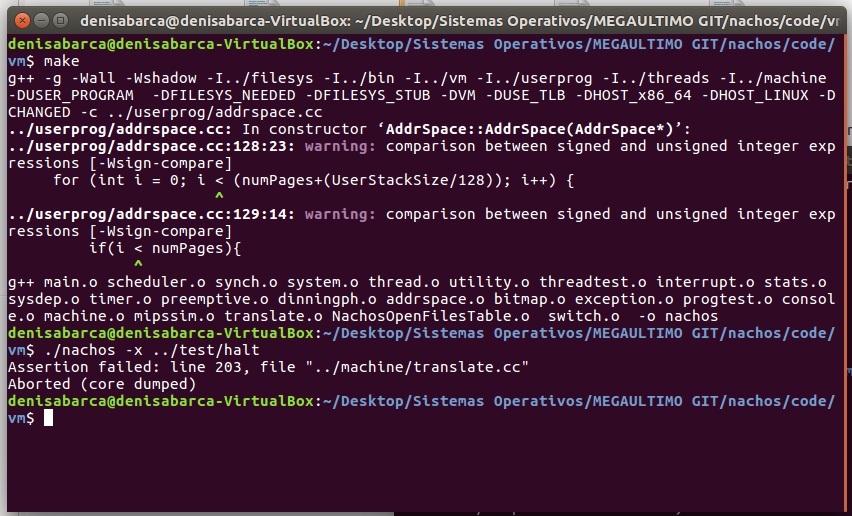
\includegraphics[width=0.5\textwidth]{Resultado_primer_Halt.PNG}
    \caption{Error de página faltante}
    \label{fig:01}
  \end{center}
\end{figure}
	  \end{enumerate}
	  
	\end{enumerate}
  \section{pageFault}
  \begin{enumerate}
    \item    Identificar y anotar en su informe cómo y cuándo es que se produce el "PageFault exception", para ello debe
    
    \begin{enumerate}
      \item para ello debe revisar el código en el archivo "machine/translate.cc" \\
      La excepción de "pagefault" se da cuando ocurre una de las 2 siguientes situaciones: se intenta acceder a una página que es más grande que la TLB o se intenta acceder a una página que no se encuentra válida.
      
      \item Para realizar las lecturas o escrituras a la memoria del procesador MIPS, el simulador utiliza los métodos "Machine::ReadMem" y "Machine::WriteMem", note que estos métodos utilizan direcciones virtuales o lógicas, anote ¿Por qué?; explicar los casos en que estos métodos retornan falso. \\
    Las dirreciónes lógicas son las direcciones que elprocesador "vería" como reales mientras que las físicas son las direcciones que se encuentran en el disco duro o memoria del computado. Este método solamente retorna falso cuando existe una excepción.
    \end{enumerate}
    \item Describir la manera cómo se emplea el TLB (Translation Look-Aside Buffer) en el procesador MIPS.\\
            Esta se emplea como un TranslationEntry de solamente 4 entradas para simular un cache. 
          
    \begin{enumerate}     
      \item Anotar la descripción de la declaración de "tlb" en "machine.h"\\
            La tlb funciona de manera parecida a la pagetable solamente que esta tiene un máximo de 4 entradas, solamente que esta es inicializada  y creada cuando se crea la clase machine, por lo que no es definida por los threads que estén corriendo.
            
      \item Explicar la iniciacilización de la variable "tlb" en "machine.cc"\\
            Esta inicialización lo que pretende es liberar la tlb y dejar limpia para su uso posterior, además de fijar el tamaño a 4 entradas. Dado que esta no puede ser cambiada.
            
      \item Revise el método "AddreSpace::RestoreState" y note que siempre se le coloca un valor a la variable "pageTable" de "machine", esto debe cambiarse porque sino "tlb" y "pageTable" de "machine" serían ambas distintos de nulo y falla unos de los "ASSERT" de "translate".\\
      \begin{lstlisting}
ifndef VM
   machine->pageTable = pageTable;
   machine->pageTableSize = numPages;
endif
      \end{lstlisting}
            
            
      \item Indicar cómo se realiza la búsqueda de la dirección virtual y anote cómo se calcula la página que la contiene, la variable "vpn"\\
      El valor del vpn se calcula mediante la dirección virtual dada dividida entre la cantidad de páginas. Esto separa la página del offset que quedaría como el residuo.
            \begin{lstlisting}
vpn = (unsigned) virtAddr / PageSize;
            \end{lstlisting}
            \begin{enumerate}
        \item Anote el procedimiento cuando el simulador utiliza la variable "pageTable" para realizar la búsqueda
              \begin{lstlisting}
if (vpn >= pageTableSize) {
    DEBUG('a', "virtual page  %d too large for page table size %d!\n", 
		virtAddr, pageTableSize);
    return AddressErrorException;
} else if (!pageTable[vpn].valid) {
    DEBUG('a', "virtual page  %d too large for page table size %d!\n", 
		virtAddr, pageTableSize);
    return PageFaultException;
}
entry = &pageTable[vpn];
              \end{lstlisting}
              \item Anote el procedimiento cuando se utiliza la variable "tlb"
              \begin{lstlisting}
for (entry = NULL, i = 0; i < TLBSize; i++)
	  if (tlb[i].valid && (tlb[i].virtualPage == vpn)) {
      entry = &tlb[i];			// FOUND!
      break;
    }
  }
              \end{lstlisting}
              \item Si la página es válida, en ambos casos se define una variable "entry", anote qué representa y cuál es su contenido lógic.\\
              Esta variable es una instancia de "pageentry" y contiene la direccion física y virtual entre otras propiedades mencionadas anteriormente
            \end{enumerate}
          \end{enumerate}
          \item  Indicar cómo se asocia la página virtual al marco de memoria física correspondiente\\
          \begin{enumerate}
            \item Explicar que representa la variable "pageFrame" en el método "Translate".\\
           La variable pageframe representa la página en donde se debe buscar la dirección ya que cuando se lee de memoria se realiza por página y no una sola dirección de memoria.
            
            \item Explicar cómo se obtiene la dirección física y cómo la devuelve este método "Translate".\\
            Para esto primeramente se obtiene el valor de la pagina y el offset, a partir del valor de
la pagina se obtiene el pageframe desde la TLB o la pagetabl, finalmente se obtiene la
direccion fisica a partir de la siguiente linea de codigo
             \begin{lstlisting}
*physAddr = pageFrame * PageSize + offset;
        \end{lstlisting}  
            \item Explicar que hace esta porción de código del método "Translate", indique en cuál estructura de datos ocurren estos cambios.\\
            \begin{lstlisting}
...
entry->use = true;		// set the use, dirty bits
if (writing)
  entry->dirty = true;
...
            \end{lstlisting}
            Estos cambios se realizan sobre pageentry, en donde se actualiza el uso de la página y además si se realiza una escritura se modifica el valor de dirty para indicar que esta página ha sido modificada.
            
            \item Explicar la funcionalidad de la bandera (bit) "dirty".\\
              Si se realiza una escritura se modifica el valor de "dirty" para indicar que esta página ha sido modificada.
            \end{enumerate}
          \item  Identificar los casos en que se produce el "PageFaultException" en el método "Translate"
          \begin{enumerate}
            \item  El simulador de MIPS no avanza los contadores de programa cuando ocurren las excepciones, en el caso de "SysCallException" lo tuvimos que hacer 'manualmente', en el caso de "PageFaultException" no hay que hacerlo, pues es indispensable que la instrucción que causó la excepción sea reejecutada.\\
            
            \item Explicar cómo va a resolver cada uno de los casos encontrados en que ocurre una excepción "PageFault"\\
            Lo  que se pretende realizar en estos casos es cargar en la memoria del tlb la página solicitada y volver el contador a la posición anterior para que la vuelva a correr.
            
          \end{enumerate}
          \item Explicar cómo va a obtener las páginas de la memoria principal para asignarlas a las páginas faltantes.
          \begin{itemize}
            \item Explicar cómo va a resolver el problema si toda la memoria física está llena.\\
            Cuando la memoria física esta llena se reliza un reemplazo de la página que fue utilizada de último con el algoritmo fifo.
            \item Explicar en que casos la página que se reemplaza debe ir a SWAP y en que caso no.\\
            En los casos en que la memoria ha sido modificada debe ir al swap y en caso contrario no.
            \item Analizar todos los casos posibles para la página que necesita ser reemplazada y su diseño de solución.\\
            
          \end{itemize}
          \item Utilización del archivo de intercambio (SWAP)
          \begin{enumerate}
            \item Explicar la estructura interna del archivo de intercambio SWAP.\\
            El archivo esta compuesto por varios bitmaps los cuales guardan la información de las páginas virtuales y las páginas físicas
            
            \item Indicar el momento en que el archivo debe construirse y destruirse.\\
            El archivo de swap se crea al crearse una nueva instancia de memoria virtual ya que este esta contenido en el constructor de dicha clase y este a su vez es llamado desde la creación del addres space
            
            \item Indicar la cantidad de elementos que este archivo debe contener.\\
            Por regla general (dada por el profesor) esta zona debe contener el doble de páginas que la memoria de pagetables osea 64 páginas de 128 bytes.
            
            \item Explicar su estrategia para que NachOS conozca cuáles de esos elementos están ocupados y cuáles están libres.\\
            Mediante el uso de bitmaps se puede lograr saber cuales están libres y cuales no.
          \end{enumerate}
    \end{enumerate}
  \section{ Características de la página faltante}
  \begin{enumerate}
    \item  Determinar cuál es la página de la dirección lógica que generó la CPU, es decir, la que provocó la excepción (PageFault exception)
    \begin{enumerate}
      \item Explicar por qué se generó esta excepción.\\
      Esta excepción se genera porque no todas las páginas del programa son cargadas al inicio, solamente lás páginas que se utilizan son las que se cargan.
      \item Averiguar cuál es la dirección que causó la excepción. Para ello debe revisar "machine.h" y la definición de los registros de la CPU, en particular ver el registro 39 \\
      \begin{lstlisting}
define BadVAddrReg	39	// The failing virtual address on an exception
      \end{lstlisting}
      Como se muestra en el código anterior, en el registro 39 se guarda la memoria que ocasiona una excepción de manejo de memoria virtual, por lo que al leerlo se obtiene dicha dirección.
      
      \item  A partir de la dirección lógica, calcular el número de página lógico necesario.\\
      La página se calcula al dividir entre la constante pagesize y el desplazamiento al obtener el módulo entre dicha constante.
      
      \item Revisar la estructura de datos "pageTable" de la variable "space" del hilo que se está ejecutando en este momento y verificar el estado de la página faltante, puede emplear rótulos informativos.\\
      Para esto se crean diferentes estados:
      \begin{lstlisting}
define En_Disco          0
define En_Memoria        1
define No_inicializado   2
      \end{lstlisting}
      
      \item     Indicar el procedimiento a seguir para lograr que no vuelva a ocurrir esa excepción de falta de página.\\
      Para que no vuelva a ocurrir dicha excepción se debe de cargar a memoria cache o tlb la página completa donde se ocacionó la excepción. y colocar el bit de use y valid en true.
      
    \end{enumerate}
  \end{enumerate}
  \section{ Actualización de estructuras}
    \begin{enumerate}
      \item Anotar los casos en que se debe cambiar el bit de validez de una página (de falso a verdadero y viceversa), indique cuales estructuras de datos deben reflejar ese cambio.\\
      En el address space se cambia la validez de una página al ser cargada se pasa a verdadero y cuando se desecha la página se debe cambiar a falso. al eliminar los hilos de un programa las páginas utilizadas pasan a un estado de validez falso
      \item Indicar cuáles estructuras debe actualizar para evitar que esa excepción ("PageFaultException") siga ocurriendo.\\
      se deben realizar cambios en el tlb y la pagetable del proceso que se esté corriendop de tal manera que se guarde la página que se intentó accesar y causó la excepción
      \item En los métodos "RestoreState" y "SaveState" indicar los cambios que considera necesarios para mantener el funcionamiento correcto de la memoria virtual de NachOS.\\
      Se debe realizar la implementación del restore state de tal manera que se cargen las páginas del tlb a pagetable del addres space y eliminar la asignación del pagetable del proceso a machine dado que ya no se debe utilizar dicha tabla sino más bien la TLB dado que esto genera un Assert.
      \begin{enumerate}
        \item Recuerde que al igual que con "pageTable" de la clase "Machine", solo vamos a tener un "tlb" que utilizan todos los hilos, el hardware modifica el TLB, pero esos cambios deben persistir en las "pageTables" de cada hilo.\\
        Para lograr esto, se debe realizar una copia del tlb de machine al pagetable del hilo de addresspace, de esta manera se garantiza que ambos poseen las mísmas páginas
        \item Explicar qué debe hacer NachOS cuando tiene que sacar un hilo de la máquina para cederlo a otro, explicar qué cambios pueden ocurrir en los datos de la TLB y en qué lugar se debe almacenar esos cambios.\\
        Cuando se realiza un swap entre 2 hilos, las páginas utilizadas por el hilo se deben de guardar en el archivo de swap, de esta manera se pueden intercambiar 2 hilos sin perder las páginas que estaban utilizando. si una página se encuentra sucia, esta debe ser guardada en memoria principal.
        \item Explicar los cambios necesarios a aplicar en los métodos anteriores para permitir ese cambio de contexto, indique cual sería el estado correcto de la TLB de la máquina cuando un proceso recién comienza a correr.\\
        Para esto se debe modificar la creación de la page table de tal manera que no se utilice ni se carge a memoria las páginas del programa, solamente se crea el page table y se rellena de falso, además se debe modificar la clase pageentry de tal manera que se pueda tener un indice para la zona de swap.
        
      \end{enumerate}
    \end{enumerate}
   \section{Actualización de información}
   \begin{enumerate}
     \item TLB
     \begin{enumerate}
       \item Indique una manera en que se puede ir llenando el TLB\\
       Al ingresar al PageFaultException, se llama al método Cargar del espacio de direcciones del proceso que recibe la posición (dirección) que requiere el proceso.
Dentro del método Cargar, se determina el índice virtual simplemente tomando la dirección solicitada y dividiéndolo por el tamaño de la página que es 128.
Se evalúa que si la página está inicializada y si está en disco. Si no está inicializada entonces se transcribe la información a memoria empleando ReadAt.
Al transferir los datos a memoria entonces se cambia la validez de la página a true tanto en el espacio de direcciones como en la TLB. Asimismo se cambia el estado de la página a $En_Memoria$.

       \item De dónde se obtiene los datos que se colocan en el TLB      
       \item Explique el algoritmo empleado para crear espacio en la TLB en caso de encontrarse llena. Para la entrega final este algoritmo ser distinto de FIFO. \\         Describa los cambios a realizar en la tabla de páginas del proceso\\
       El código donde se implementó el procedimiento es el siguiente:
        \begin{lstlisting}
int AddrSpace::Cargar(int virtualIndex)
{       
int resultado = -1;  
// virtualIndex  =1;
//Guardo el estado de la pagina
int estado = pageTable[virtualIndex].state;
//Si la pagina no esta inicializada o esta en el disco
if(estado == No_inicializado || estado == En_Disco){
//Asigna la pagina en el dico
resultado = pageTable[virtualIndex].physicalPage = 
virtualMem->setPaginaDisco(this);

if(resultado != -1){

//Si esta en el disco
if(estado == En_Disco)
{		
//Traiga la pagina del disco y pongala en memoria
virtualMem->getPaginaDisco(this, virtualIndex);
//Si no esta inicializada
}
else
//Lea la pagina de memoria y cargue la pagina
programa->ReadAt(&(machine->mainMemory[pageTable[virtualIndex].physicalPage
* PageSize]), PageSize, inicioCodigo + virtualIndex * PageSize);
//Indica que la pagina es valida en este momento
pageTable[virtualIndex].valid = true;
//Indica que la pagina se encuentra en memoria en este momento
pageTable[virtualIndex].state = En_Memoria;
}
}
if(pageTable[virtualIndex].state == En_Memoria){
int i=0;
while(machine->tlb[i].use){
machine->tlb[i].use = false;
if(i < TLBSize)
i++;
else
i=0;
}
machine->tlb[i] = pageTable[virtualIndex];
resultado = machine->tlb[i].physicalPage;
}
return resultado;
}
        \end{lstlisting}

     \end{enumerate}
   \end{enumerate}
\section{Pruebas finales}  
\begin{enumerate}
  \item  Verifique el programa "halt" funcione, debe hacer 3 faltas:
    \begin{itemize}
      \item         0, en la página 0
       \item   208, en la página 1
        \item 1260, en la página 9

    \end{itemize}
    Al  probar el método Halt se obtuvo el siguiente de la figura \ref{fig:02}.\\
    \begin{figure}[b]
  \begin{center}
    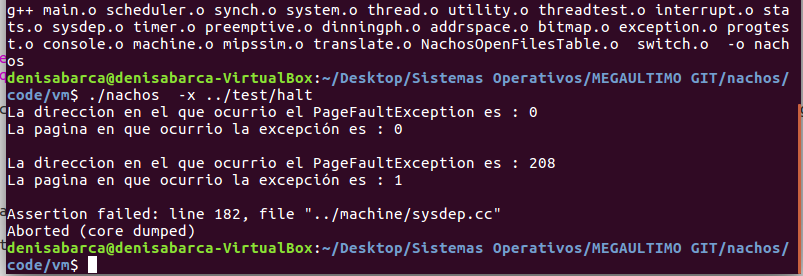
\includegraphics[width=0.5\textwidth]{Resultado_final_Halt.PNG}
    \caption{Prueba Halt }
    \label{fig:02}
  \end{center}
\end{figure}
Se observa que las primeras dos páginas y direcciones las ejecuta de manera correcta, sin embargo falla en un punto de validación (Assertion point) y no se ejecuta la última página. Lo anterior puede deberse a un fallo en las condiciones en que se ingresa a la excepción PageFaultException.
\end{enumerate}
    
\end{document}
